%67
\subsection{Elem törlése kétszeresen láncolt listából}
\begin{frame}
  \begin{center}
    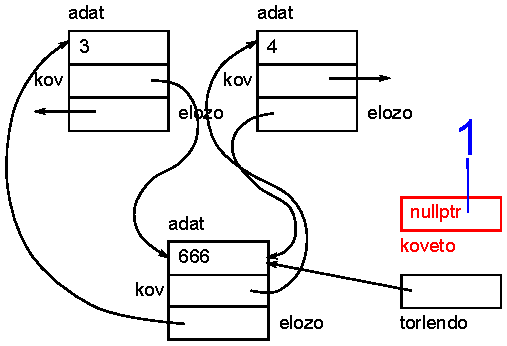
\includegraphics[scale=0.55]{lista2/list2-10.pdf}
  \end{center}
  \vspace{-.4cm}
  \scriptsize
  \begin{exampleblock}{\textattachfile{Lista2.cpp}{Lista2.cpp}}
    \tiny
    \vspace{-.2cm}
    \lstinputlisting[style=cpp,linerange={30-40},numbers=left,firstnumber=30]{Lista2.cpp}
    \vspace{-.2cm}
  \end{exampleblock}
\end{frame}

%68
\begin{frame}
  \begin{center}
    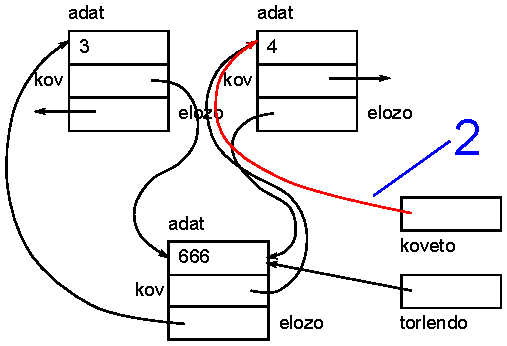
\includegraphics[scale=0.55]{lista2/list2-11.pdf}
  \end{center}
  \vspace{-.4cm}
  \scriptsize
  \begin{exampleblock}{\textattachfile{Lista2.cpp}{Lista2.cpp}}
    \tiny
    \vspace{-.2cm}
    \lstinputlisting[style=cpp,linerange={30-40},numbers=left,firstnumber=30]{Lista2.cpp}
    \vspace{-.2cm}
  \end{exampleblock}
\end{frame}

%69
\begin{frame}
  \begin{center}
    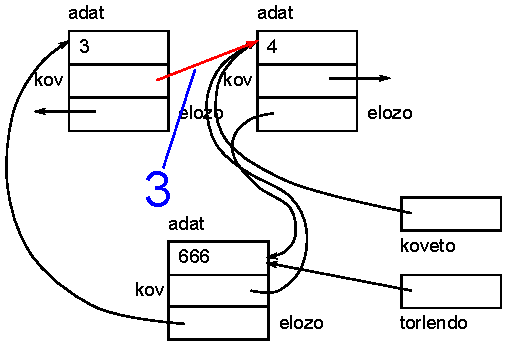
\includegraphics[scale=0.55]{lista2/list2-12.pdf}
  \end{center}
  \vspace{-.4cm}
  \scriptsize
  \begin{exampleblock}{\textattachfile{Lista2.cpp}{Lista2.cpp}}
    \tiny
    \vspace{-.2cm}
    \lstinputlisting[style=cpp,linerange={30-40},numbers=left,firstnumber=30]{Lista2.cpp}
    \vspace{-.2cm}
  \end{exampleblock}
\end{frame}

%70
\begin{frame}
  \begin{center}
    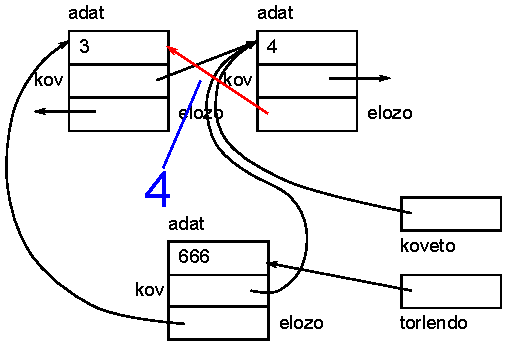
\includegraphics[scale=0.55]{lista2/list2-13.pdf}
  \end{center}
  \vspace{-.4cm}
  \scriptsize
  \begin{exampleblock}{\textattachfile{Lista2.cpp}{Lista2.cpp}}
    \tiny
    \vspace{-.2cm}
    \lstinputlisting[style=cpp,linerange={30-40},numbers=left,firstnumber=30]{Lista2.cpp}
    \vspace{-.2cm}
  \end{exampleblock}
\end{frame}

%71
\begin{frame}
  \begin{center}
    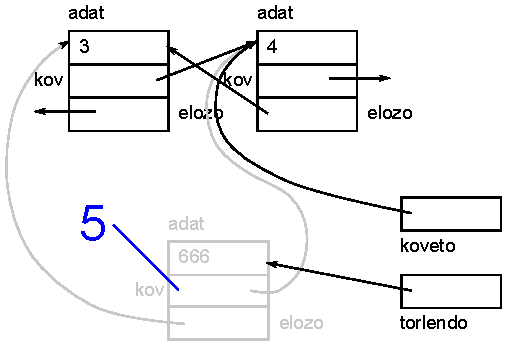
\includegraphics[scale=0.55]{lista2/list2-14.pdf}
  \end{center}
  \vspace{-.4cm}
  \scriptsize
  \begin{exampleblock}{\textattachfile{Lista2.cpp}{Lista2.cpp}}
    \tiny
    \vspace{-.2cm}
    \lstinputlisting[style=cpp,linerange={30-40},numbers=left,firstnumber=30]{Lista2.cpp}
    \vspace{-.2cm}
  \end{exampleblock}
\end{frame}

%72
\begin{frame}
  \begin{center}
    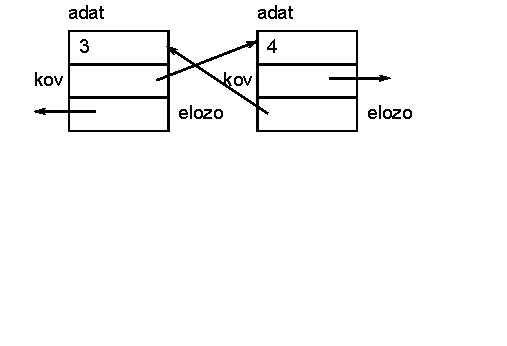
\includegraphics[scale=0.55]{lista2/list2-15.pdf}
  \end{center}
  \vspace{-.4cm}
  \scriptsize
  \begin{exampleblock}{\textattachfile{Lista2.cpp}{Lista2.cpp}}
    \tiny
    \vspace{-.2cm}
    \lstinputlisting[style=cpp,linerange={30-40},numbers=left,firstnumber=30]{Lista2.cpp}
    \vspace{-.2cm}
  \end{exampleblock}
\end{frame}